\chapter{Layout of the circuit} \label{app:blocks}
This purpose of this chapter is to give an overview of what the circuit is 
supposed to look like, realized using blocks. The top entity is the 
aes\_scrambler (Figure \ref{block:scrambler}). Note that the manager-entity in Figure \ref{block:scrambler} and 
\ref{block:round} are not the same entities.

\begin{figure}
  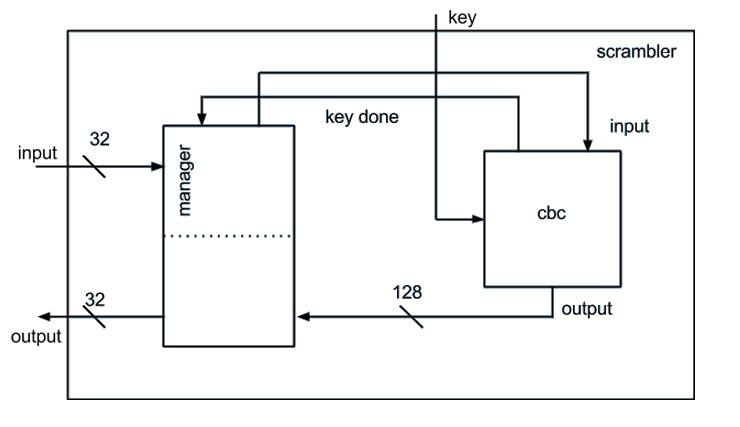
\includegraphics[width=\textwidth]{scrambler}
  \caption{Scrambler-block}
  \label{block:scrambler}
\end{figure}

\begin{figure}
  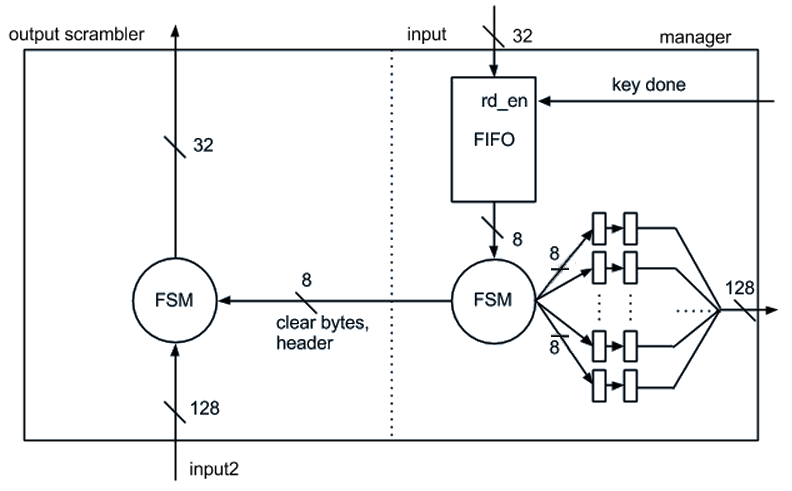
\includegraphics[width=\textwidth]{manager}
  \caption{Manager-block}
  \label{block:manager}
\end{figure}

\begin{figure}
  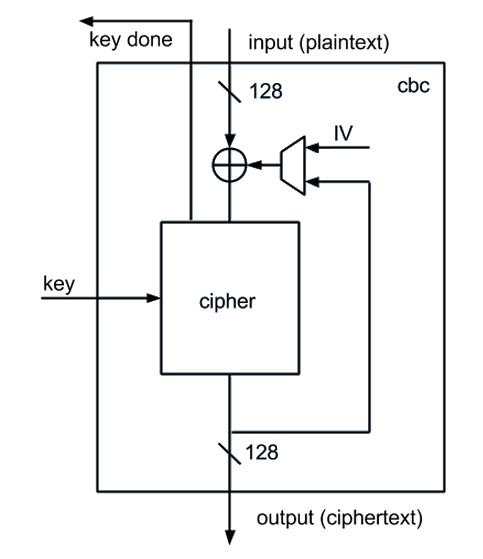
\includegraphics[width=\textwidth]{cbc}
  \caption{CBC-block}
  \label{block:cbc}
\end{figure}

\begin{figure}
  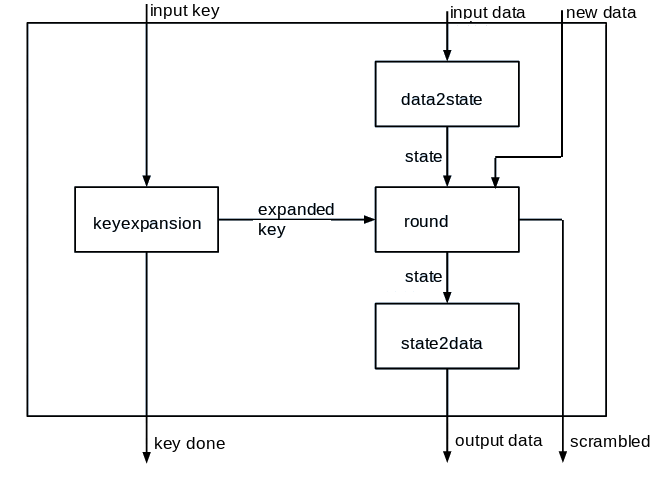
\includegraphics[width=\textwidth]{cipherblock}
  \caption{Cipher-block}
  \label{block:cipher}
\end{figure}

\begin{figure}
  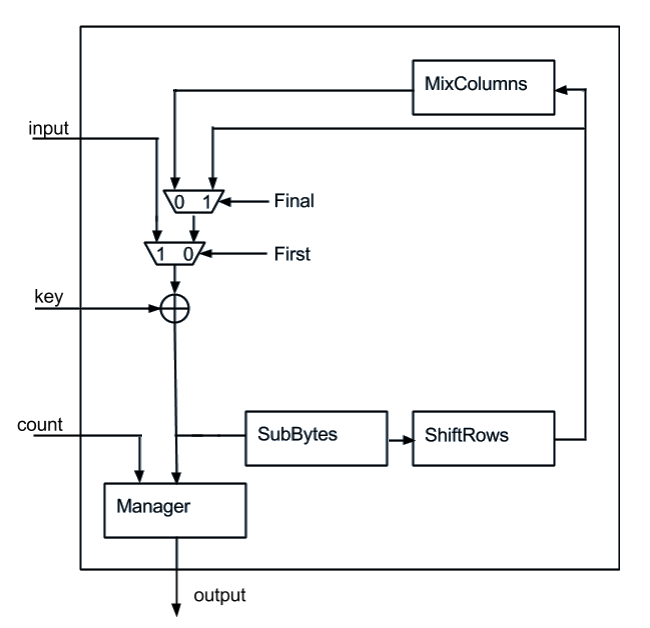
\includegraphics[width=\textwidth]{round}
  \caption{Round-block}
  \label{block:round}
\end{figure}
